\documentclass[11pt, a4paper]{article} % setsfont size and layout

%% required packages %%

\usepackage[margin=2.5cm]{geometry} % margins
\usepackage[utf8]{inputenc} % Umlaute
\usepackage{amsmath,amssymb, physics}		% math formulas
\usepackage{graphicx}		% graphics
\usepackage{fancyhdr}		% header and footer on every page
\usepackage{setspace}		% line space (e.g. \singlespacing, \onehalfspacing or \doublespacing)

\usepackage{braket}
\usepackage{xcolor}
%% Here the main part of the document begins %%

\begin{document}
	
%% Some more settings %%
	
\setlength{\parindent}{0pt} % first line in paragraph will not be indented
\onehalfspacing				% 1.5 line spacing
%\thispagestyle{empty}		% no header and page number on first page


%% Header on first page with course information etc. %%
%\begin{tabular}{p{15.5cm}}
%	{\large \textbf{Classical Mechanics}} \\
%	Westlake University \\ 
%	\hline
%	\\
%\end{tabular}

\vspace*{0.1cm}				% vertical space between header on top of the page and main heading


\begin{center}
	{\Large \textbf{Classical Mechanics}}
    \vspace*{2mm}
    
    {\Large \textbf{Final Exam}}
	\vspace{8mm}
%Name: 
%\end{center} 
%\vspace{0.1cm}

{\Large \bf \color{red} Time: 2:00 - 4:00 pm, Dec. 30th, 2025}
\vspace*{2mm}

{\Large \bf \color{red} Duration: 120 minutes}
\vspace*{2mm}

{\Large \bf \color{red} Total Points: 100}
\end{center}
\vspace*{8mm}

{\Large \bf \color{orange} Instruction:} 
\vspace*{2mm}

{\Large \bf \color{orange} \hspace{2em} This is a closed-book exam; no aids are allowed.}
\vspace*{2mm}

{\Large \bf \color{orange} \hspace{2em} Total 10 pages including the front page of the instruction.}
\vspace*{2mm}

{\Large \bf \color{orange} \hspace{2em} Provide relevant mathematical steps.} 
\vspace*{2mm}

{\Large \bf \color{orange} \hspace{2em} All answers must be in English.}
\vspace*{2mm}

{\Large \bf \color{orange} \hspace{2em} Don't open the booklet before the exam begins.}
\vspace{5cm}

\begin{center}
{\Large \bf Student Name: \underline{\hbox to 40mm{}}}
\vspace*{8mm}

{\Large \bf Student ID: \underline{\hbox to 40mm{}}}
\vspace*{2mm}
\end{center}

\newpage
\section*{Problem 1 [$5 + 5$ points]} 
\begin{enumerate}
  \item[(1)] Write down Newton’s second law, the Euler-Lagrange equation, and Hamilton’s equations of motion. 

  \item[(2)] Using $S=\int_{t_i}^{t_f}(\dot{q}p-H )\dd t$ and the Least Action Principle to derive the Hamiton's equations of motion.

  \end{enumerate}

\subsection*{Answer}

\subsubsection*{(1) Fundamental Equations [5 points]}

\begin{description}
    \item[A. Newton's Second Law] \hfill \textbf{[1 point]}
    \begin{itemize}
        \item Equation: $\mathbf{F} = \frac{d\mathbf{p}}{dt}$ or $\mathbf{F} = m\mathbf{a}$ (or $\mathbf{F} = m\ddot{\mathbf{r}}$).
        \item \textit{Note:} Vector notation ($\mathbf{F}, \mathbf{a}$) or component index notation ($F_i = m \ddot{x}_i$) is required. If scalar form is written without context, deduct 0.5 points.
    \end{itemize}

    \item[B. Euler-Lagrange Equation] \hfill \textbf{[2 points]}
    \begin{itemize}
        \item Equation: $\frac{d}{dt}\left(\frac{\partial L}{\partial \dot{q}_i}\right) - \frac{\partial L}{\partial q_i} = 0$ (for $i = 1, \dots, n$).
    \end{itemize}

    \item[C. Hamilton's Equations of Motion] \hfill \textbf{[2 points]}
    \begin{itemize}
        \item Equations: 
        \begin{align*}
            \dot{q}_i &= \frac{\partial H}{\partial p_i} \\
            \dot{p}_i &= -\frac{\partial H}{\partial q_i}
        \end{align*}
    \end{itemize}
\end{description}

\subsubsection*{(2) Derivation via Least Action Principle [5 points]}
\begin{description}
    \item[A. Variation Setup] \hfill \textbf{[1 point]}
    \begin{itemize}
        \item Define the variation of the action $S = \int_{t_i}^{t_f} (\dot{q}p - H) dt$.
        \item Substitute perturbed paths into the integral:
        $$ q \to q + \varepsilon, \quad p \to p + \tilde{\varepsilon} $$
        (Standard notation $\delta q$ and $\delta p$ is also acceptable).
        \item Equation setup:
        $$ S[\text{varied}] = \int_{t_i}^{t_f} dt \left[ (p+\tilde{\varepsilon})\frac{d}{dt}(q+\varepsilon) - H(p+\tilde{\varepsilon}, q+\varepsilon) \right] $$
    \end{itemize}

    \item[B. Expansion and Linearization] \hfill \textbf{[1 point]}
    \begin{itemize}
        \item Taylor expand the Hamiltonian to first order and expand the product term:
        $$ H(p+\tilde{\varepsilon}, q+\varepsilon) \approx H + \frac{\partial H}{\partial p}\tilde{\varepsilon} + \frac{\partial H}{\partial q}\varepsilon $$
        \item Group terms linear in $\varepsilon$ and $\tilde{\varepsilon}$:
        $$ \delta S = \int_{t_i}^{t_f} dt \left[ p\dot{\varepsilon} + \tilde{\varepsilon}\dot{q} - \frac{\partial H}{\partial p}\tilde{\varepsilon} - \frac{\partial H}{\partial q}\varepsilon \right] $$
    \end{itemize}

    \item[C. Integration by Parts] \hfill \textbf{[1.5 points]}
    \begin{itemize}
        \item Transform the term involving $\dot{\varepsilon}$ (or $\delta \dot{q}$) using integration by parts:
        $$ \int_{t_i}^{t_f} p \frac{d\varepsilon}{dt} dt = \left[ p\varepsilon \right]_{t_i}^{t_f} - \int_{t_i}^{t_f} \dot{p} \varepsilon dt $$
        \item \textbf{Boundary Condition:} Explicitly state that the boundary term vanishes because variations at endpoints are zero ($\varepsilon(t_i)=\varepsilon(t_f)=0$).
        \item Resulting variation integral:
        $$ \delta S = \int_{t_i}^{t_f} dt \left[ \tilde{\varepsilon}\left(\dot{q} - \frac{\partial H}{\partial p}\right) - \varepsilon\left(\dot{p} + \frac{\partial H}{\partial q}\right) \right] $$
    \end{itemize}

    \item[D. Independence Argument and Conclusion] \hfill \textbf{[1.5 points]}
    \begin{itemize}
        \item \textbf{Independence Argument [0.5 pt]:} State that $\varepsilon$ (variation in $q$) and $\tilde{\varepsilon}$ (variation in $p$) are completely \textbf{independent} variations.
        \item \textbf{Final Equations [1 pt]:} Conclude that the coefficients of $\varepsilon$ and $\tilde{\varepsilon}$ must vanish separately:
        $$ \dot{q} = \frac{\partial H}{\partial p}, \quad \dot{p} = -\frac{\partial H}{\partial q} $$
    \end{itemize}
\end{description}

\newpage 
\section*{Problem 2 [$10$ points]} 
A particle of mass $m$ is attracted to the origin by a force of magnitude $k/r^2$. Using plane polar coordinates, find the Hamiltonian and Hamilton's equations of motion. Sketch constant-$H$ contours in the $(r,p_r)$ phase plane.

\subsection*{Answer}

\subsubsection*{(1) The Hamiltonian [5 points]}
\begin{description}
    \item[A. Lagrangian Setup] \hfill \textbf{[2 points]}
    \begin{itemize}
        \item Correctly identifying Kinetic Energy in polar coordinates: $T = \frac{1}{2}m(\dot{r}^2 + r^2\dot{\theta}^2)$. \textbf{[1 point]}
        \item Correctly identifying Potential Energy for an attractive force: $U(r) = -k/r$. \textbf{[1 point]}
    \end{itemize}

    \item[B. Canonical Momenta] \hfill \textbf{[1 point]}
    \begin{itemize}
        \item Deriving momenta from the Lagrangian ($L=T-U$):
        \[ p_r = \frac{\partial L}{\partial \dot{r}} = m\dot{r}, \quad p_\theta = \frac{\partial L}{\partial \dot{\theta}} = mr^2\dot{\theta} \]
    \end{itemize}

    \item[C. The Hamiltonian Function] \hfill \textbf{[2 points]}
    \begin{itemize}
        \item Definition: $H = \sum \dot{q}p - L$ or recognizing $H = T+U$ (for conservative, scleronomic systems).
        \item \textbf{Final Expression:} Expressing $H$ strictly in terms of coordinates and \textbf{momenta} (not velocities):
        \[ H(r, \theta, p_r, p_\theta) = \frac{p_r^2}{2m} + \frac{p_\theta^2}{2mr^2} - \frac{k}{r} \]
    \end{itemize}
\end{description}

\subsubsection*{(2) Hamilton's Equations of Motion [3 points]}
\begin{description}
    \item[A. Coordinate Derivatives] \hfill \textbf{[1 point]}
    \begin{align*}
        \dot{r} &= \frac{\partial H}{\partial p_r} = \frac{p_r}{m} \\
        \dot{\theta} &= \frac{\partial H}{\partial p_\theta} = \frac{p_\theta}{mr^2}
    \end{align*}
    
    \item[B. Momentum Derivatives] \hfill \textbf{[2 points]}
    \begin{itemize}
        \item Equation for $p_\theta$:
        \[ \dot{p}_\theta = -\frac{\partial H}{\partial \theta} = 0 \implies p_\theta = \text{const} \]
        \textbf{[1 point]}
        \item Equation for $p_r$:
        \[ \dot{p}_r = -\frac{\partial H}{\partial r} = \frac{p_\theta^2}{mr^3} - \frac{k}{r^2} \]
        \textbf{[1 point]}
    \end{itemize}
\end{description}

\subsubsection*{(3) Phase Plane Sketch [2 points]}
\begin{description}
    \item[A. Phase Curve Equation/Analysis] \hfill \textbf{[1 point]}
    \begin{itemize}
        \item Rearranging the energy equation to express $p_r$ as a function of $r$:
        \[ p_r(r) = \pm \sqrt{2m\left(H + \frac{k}{r} - \frac{p_\theta^2}{2mr^2}\right)} \]
        \item Or a qualitative analysis of the effective potential $V_{eff} = -k/r + p_\theta^2/(2mr^2)$.
    \end{itemize}

    \item[B. Sketch of Contours] \hfill \textbf{[1 point]}
    \begin{itemize}
        \item Sketching curves in the $(r, p_r)$ plane.
        \begin{figure}[h]
            \centering
            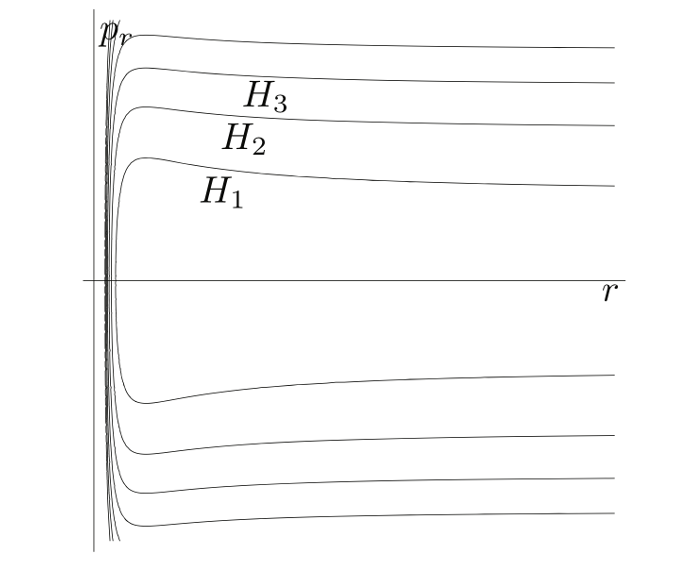
\includegraphics[width=0.5\textwidth]{p2-anw.png}
            \label{P7}
        \end{figure}
    \end{itemize}
\end{description}

\newpage
\section*{Problem 3 [$10$ points]}
A bead of mass $m$ slides on a frictionless rod inclined at a constant angle $\alpha$ to the vertical axis. The rod rotates about this vertical axis with a constant angular velocity $\omega$. Gravity $g$ acts vertically downwards. Derive the equation of motion for the position $r$ of the bead along the rod using the Lagrangian formalism. 
\begin{figure}[h]
    \centering
    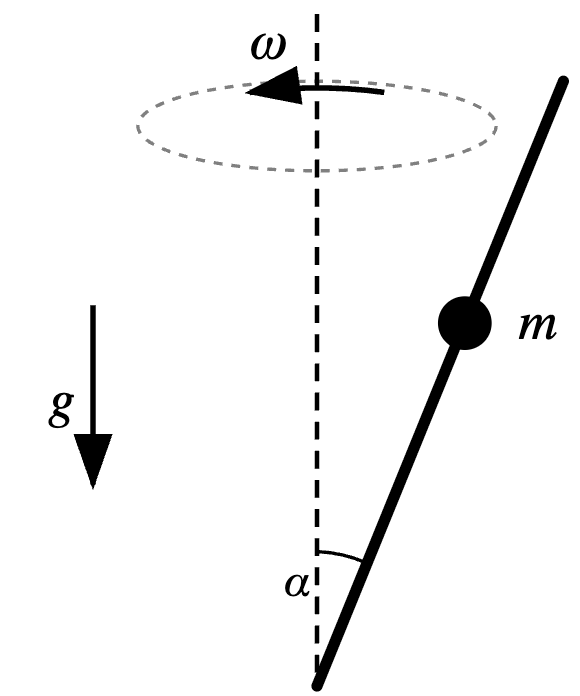
\includegraphics[width=0.35\textwidth]{bead.png}
    \label{P7}
\end{figure}

\subsection*{Answer}

\subsubsection*{(a) Lagrangian Formulation (5 points)}
\begin{itemize}
    \item \textbf{Kinetic Energy ($T$):} Identify the velocity components. The radial velocity is $\dot{r}$ and the tangential velocity due to rotation is $\omega(r \sin \alpha)$.
    \[
    T = \frac{1}{2}m v^2 = \frac{1}{2}m \left( \dot{r}^2 + (\omega r \sin \alpha)^2 \right)
    \]
    \hfill \textbf{(2 points)} \\

    \item \textbf{Potential Energy ($V$):} Define the gravitational potential energy based on the height $h = r \cos \alpha$ (assuming $V=0$ at $r=0$).
    \[
    V = m g r \cos \alpha
    \]
    \hfill \textbf{(2 points)}

    \item \textbf{The Lagrangian ($L$):} Construct the Lagrangian $L = T - V$.
    \[
    L = \frac{1}{2}m(\dot{r}^2 + \omega^2 r^2 \sin^2 \alpha) - m g r \cos \alpha
    \]
    \hfill \textbf{(1 point)}
\end{itemize}

\subsubsection*{(b) Equation of Motion (5 points)}
\begin{itemize}
    \item \textbf{Derivatives:} Calculate the necessary partial derivatives for the Euler-Lagrange equation $\frac{d}{dt}(\frac{\partial L}{\partial \dot{r}}) - \frac{\partial L}{\partial r} = 0$.
    \[
    \frac{\partial L}{\partial \dot{r}} = m\dot{r} \implies \frac{d}{dt}\left(\frac{\partial L}{\partial \dot{r}}\right) = m\ddot{r}
    \]
    \[
    \frac{\partial L}{\partial r} = m \omega^2 r \sin^2 \alpha - m g \cos \alpha
    \]
    \hfill \textbf{(3 points)} \\

    \item \textbf{Final Equation:} Assemble and rearrange the terms to obtain the final equation of motion.
    \[
    m\ddot{r} - (m \omega^2 r \sin^2 \alpha - m g \cos \alpha) = 0
    \]
    \[
    \implies m\ddot{r} = m \omega^2 r \sin^2 \alpha - m g \cos \alpha
    \]
    \hfill \textbf{(2 points)} \\
\end{itemize}

\newpage
\section*{Problem 4 [$10$ points]}
Consider the simple harmonic oscillator, with a particle of mass $m$ free to move in one dimension, connected to a spring with Hamiltonian

\begin{equation*}
    H = \frac{p^2}{2m} + \frac{1}{2}m\omega^2q^2
\end{equation*}

where $\omega = \sqrt{k/m}$ is the natural angular frequency and $k$ is the spring constant. The phase space is two-dimensional, parameterized by \{$q$, $p$\}. Let us apply the canonical transformation defined as

\begin{equation*}
    F_1(q, Q, t) = qQ.
\end{equation*}

\begin{enumerate}
\item[(1)] Find the new Hamiltonian after the canonical transformation

\item[(2)]  Is following transformation a canonical transformation? Calculate the Poisson bracket to justify your answer. 

\begin{equation*}
    q(Q, P) = \sqrt{\frac{2P}{m\omega}}\sin{Q},\ p(Q, P) = \sqrt{2m\omega P}\cos{Q}.
\end{equation*}
\end{enumerate}

\subsection*{Answer}

\subsubsection*{(1) New Hamiltonian via Generating Function [4 points]}
\begin{itemize}
    \item \textbf{Transformation Relations:} \hfill \textbf{(2 points)} \\
    State or apply the standard relations for a Type 1 generating function $F_1(q, Q)$:
    \[ p = \frac{\partial F_1}{\partial q}, \quad P = - \frac{\partial F_1}{\partial Q} \]
    Substitute $F_1 = qQ$ to find the explicit relationships:
    \[ p = Q, \quad P = -q \implies q = -P \]

    \item \textbf{Construct New Hamiltonian:} \hfill \textbf{(2 points)} \\
    Since $F_1$ does not depend explicitly on time, the new Hamiltonian $K$ equals the old Hamiltonian $H$:
    \[ K(Q, P) = H(q(Q, P), p(Q, P)) \]
    Substitute $q = -P$ and $p = Q$ into the original expression $H = \frac{p^2}{2m} + \frac{1}{2}m\omega^2 q^2$:
    \[ K(Q, P) = \frac{Q^2}{2m} + \frac{1}{2}m\omega^2 (-P)^2 = \frac{Q^2}{2m} + \frac{1}{2}m\omega^2 P^2 \]
\end{itemize}

\subsubsection*{(2) Poisson Bracket Verification [6 points]}
\begin{itemize}
    \item \textbf{Condition for Canonical Transformation:} \hfill \textbf{(1 point)} \\
    State that for the transformation to be canonical, the fundamental Poisson bracket must be unity:
    \[ [q, p]_{Q, P} = \frac{\partial q}{\partial Q}\frac{\partial p}{\partial P} - \frac{\partial q}{\partial P}\frac{\partial p}{\partial Q} = 1 \]

    \item \textbf{Calculate Partial Derivatives:} \hfill \textbf{(2 points)} \\
    Compute the four partial derivatives required for the bracket:
    \[ \frac{\partial q}{\partial Q} = \sqrt{\frac{2P}{m\omega}}\cos Q, \quad \frac{\partial p}{\partial P} = \sqrt{\frac{m\omega}{2P}}\cos Q \]
    \[ \frac{\partial q}{\partial P} = \frac{1}{\sqrt{2Pm\omega}}\sin Q, \quad \frac{\partial p}{\partial Q} = -\sqrt{2m\omega P}\sin Q \]

    \item \textbf{Evaluate the Bracket:} \hfill \textbf{(2 points)} \\
    Substitute the derivatives into the Poisson bracket formula:
    \begin{align*}
        [q, p] &= \left(\sqrt{\frac{2P}{m\omega}}\cos Q\right)\left(\sqrt{\frac{m\omega}{2P}}\cos Q\right) - \left(\frac{1}{\sqrt{2Pm\omega}}\sin Q\right)\left(-\sqrt{2m\omega P}\sin Q\right) \\
        &= \left( \cos^2 Q \right) - \left( -\sin^2 Q \right) \\
        &= \cos^2 Q + \sin^2 Q
    \end{align*}

    \item \textbf{Conclusion:} \hfill \textbf{(1 point)} \\
    State the final result and conclusion clearly:
    \[ [q, p] = 1 \]
    Therefore, the transformation \textbf{is canonical}.
\end{itemize}

\newpage
\section*{Problem 5 [$10$ points]}
A pendulum consists of a mass $m$ and a massless stick of length $l$. The pendulum support oscillates horizontally with a position given by $x(t) = A \cos(wt)$ (represented by a double-headed arrow in the figure below). What is the general solution for the angle of the pendulum as a function of time?

\begin{figure}[h]
    \centering
    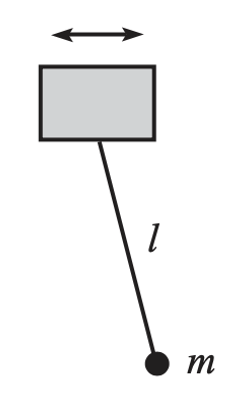
\includegraphics[width=0.25\textwidth]{Finala_P8.png}
    \label{P7}
\end{figure}

\subsection*{Answer}

\subsubsection*{(1) Kinematics and Lagrangian [3 points]}
\begin{description}
    \item[A. Coordinate Definition and Velocity] \hfill \textbf{[1 point]}
    \begin{itemize}
        \item Define the position of mass $m$: $(X, Y) = (x(t) + l\sin\theta, -l\cos\theta)$.
        \item Calculate the square of velocity $V^2 = \dot{X}^2 + \dot{Y}^2$:
        $$ V^2 = l^2\dot{\theta}^2 + \dot{x}^2 + 2l\dot{x}\dot{\theta}\cos\theta $$
    \end{itemize}
    \item[B. The Lagrangian] \hfill \textbf{[2 points]}
    \begin{itemize}
        \item Construct the Lagrangian $L = T - V$:
        $$ L = \frac{1}{2}m(l^2\dot{\theta}^2 + \dot{x}^2 + 2l\dot{x}\dot{\theta}\cos\theta) + mgl\cos\theta $$
    \end{itemize}
\end{description}

\subsubsection*{(2) Equation of Motion [2 points]}
\begin{description}
    \item[A. Application of Euler-Lagrange Equation] \hfill \textbf{[1 point]}
    \begin{itemize}
        \item Apply $\frac{d}{dt}\left(\frac{\partial L}{\partial \dot{\theta}}\right) - \frac{\partial L}{\partial \theta} = 0$:
        $$ \frac{d}{dt}(ml^2\dot{\theta} + ml\dot{x}\cos\theta) = -ml\dot{x}\dot{\theta}\sin\theta - mgl\sin\theta $$
    \end{itemize}
    \item[B. Exact Equation of Motion] \hfill \textbf{[1 point]}
    \begin{itemize}
        \item Simplify derivatives and plug in $\ddot{x} = -A\omega^2 \cos(\omega t)$ to obtain the exact differential equation:
        $$ l\ddot{\theta} - A\omega^2 \cos(\omega t) \cos\theta + g\sin\theta = 0 $$
    \end{itemize}
\end{description}

\subsubsection*{(3) Small Angle Approximation [2 points]}
\begin{description}
    \item[A. Linearization] \hfill \textbf{[1 point]}
    \begin{itemize}
        \item Apply approximations for small $\theta$: $\sin\theta \approx \theta$ and $\cos\theta \approx 1$.
        \item Explicitly state or apply that the term $\cos\theta \cos(\omega t) \approx \cos(\omega t)$.
    \end{itemize}
    \item[B. Driven Oscillator Equation] \hfill \textbf{[1 point]}
    \begin{itemize}
        \item Obtain the linear differential equation of a driven harmonic oscillator:
        $$ \ddot{\theta} + \omega_0^2 \theta = \frac{A}{l}\omega^2 \cos(\omega t) $$
        where $\omega_0 = \sqrt{g/l}$.
    \end{itemize}
\end{description}

\subsubsection*{(4) General Solution [3 points]}
\begin{description}
    \item[A. Homogeneous Solution] \hfill \textbf{[1 point]}
    \begin{itemize}
        \item Identify the transient (free oscillation) part of the solution:
        $$ \theta_h(t) = C \cos(\omega_0 t + \phi) $$
        \textit{Note: $A\sin(\omega_0 t) + B\cos(\omega_0 t)$ is also acceptable.}
    \end{itemize}
    \item[B. Particular Solution] \hfill \textbf{[2 points]}
    \begin{itemize}
        \item Identify the steady-state (driven) part of the solution ansatz $\theta_p(t) = B \cos(\omega t)$.
        \item Correctly determine the amplitude coefficient:
        $$ \theta_p(t) = \frac{A}{l} \frac{\omega^2}{\omega_0^2 - \omega^2} \cos(\omega t) $$
    \end{itemize}
    \item[Final Result Check:] The total solution is the sum of A and B.
    $$ \theta(t) = \frac{A \omega^2}{g - l\omega^2} \cos(\omega t) + C \cos\left(\sqrt{\frac{g}{l}}t + \phi\right) $$
\end{description}

% \newpage
% \section*{Problem 6 [$10$ points]}
% Assume $H(q_1, q_2, p_1, p_2)=q_1p_1 -q_2p_2-aq_1^2 + bq_2^2$, where $a$ and $b$ are constants. Calculate the total time derivative of $q_1q_2$.


\newpage

\section*{Problem 6 [$6+6$ points]}
A satellite of mass $m$ carrying a crew is initially in a stable circular orbit (Orbit 1) of radius $R_1$ around a central body of mass $M$. The crew wishes to transfer the satellite to a larger circular orbit (Orbit 3) with a radius of $R_3 = 2R_1$. To achieve this, they perform a maneuver involving two successive impulsive boosts. 
First, the satellite performs an initial boost that increases its velocity instantaneously, placing it onto an elliptical transfer orbit (denoted as Orbit 2). This transfer orbit has its perigee at radius $R_1$ (the radius of the initial circular orbit) and its apogee at $R_3 = 2R_1$.
Next, upon reaching the apogee of the transfer orbit (point $P'$), the satellite performs a second instantaneous velocity change. This second boost increases the satellite's speed such that it transitions into a final circular orbit of radius $2R_1$.
\begin{enumerate}
    \item[(1)] Determine the thrust factor $\lambda$ required for the first boost, defined as the ratio of the speed after the boost to the speed before the boost ($\lambda = v_{p} / v_1$).
    \item[(2)] Determine the thrust factor $\lambda'$ required for the second boost, defined as the ratio of the speed after the boost to the speed before the boost ($\lambda' = v_3 / v_{p'}$).
\end{enumerate}

\textbf{Hint:} The orbit of a satellite is given by $
r(\phi) = \frac{c}{1 + \epsilon \cos \phi}$. 
$\epsilon$ is the eccentricity of the orbit; $c = \frac{L^2}{GMm^2}$, where $L$ is the satellite’s angular momentum.

\begin{figure}[h]
    \centering
    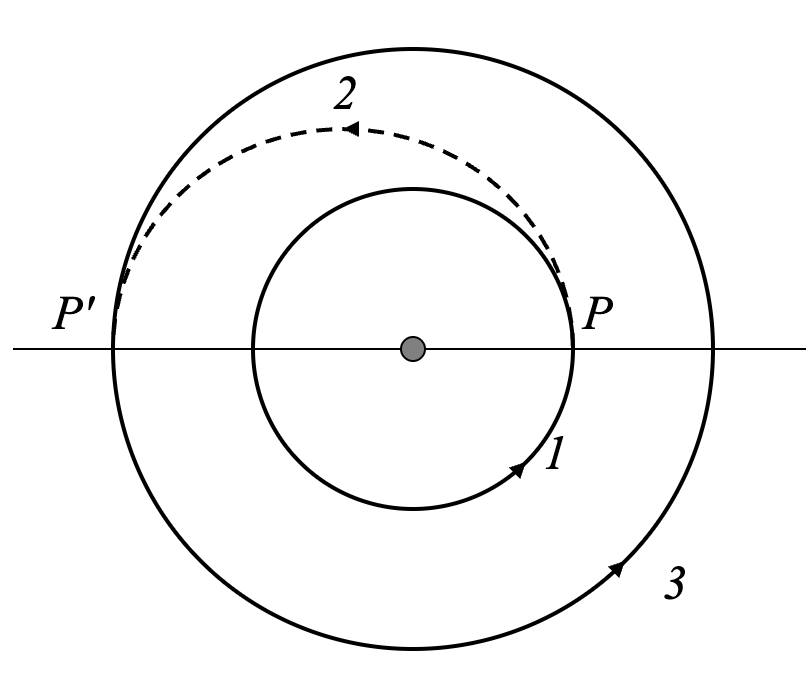
\includegraphics[width=0.3\textwidth]{transfer.png}
    \label{P7}
\end{figure}

\subsection*{Answer}

\subsubsection*{(1) Thrust factor $\lambda$ for the first boost (6 points)}
\begin{itemize}
    \item \textbf{Identify parameters for the initial circular orbit and transfer orbit:} \\
    For the initial circular orbit (Orbit 1), $c_1 = R_1$ and $\epsilon_1 = 0$. \\
    Since the velocity is boosted by $\lambda$ ($v_p = \lambda v_1$) at the same radius $R_1$, and given $c \propto L^2 \propto v^2$, the parameter $c_2$ for the transfer orbit is:
    \[
    c_2 = \lambda^2 c_1 = \lambda^2 R_1
    \]
    \hfill \textbf{(2 points)}

    \item \textbf{Relate eccentricity $\epsilon_2$ to $\lambda$ at perigee ($P$):} \\
    Point $P$ is the perigee of the transfer orbit. Using the orbit equation at $\phi=0$:
    \[
    R_1 = \frac{c_2}{1 + \epsilon_2} \implies 1 + \epsilon_2 = \frac{\lambda^2 R_1}{R_1} = \lambda^2 \implies \epsilon_2 = \lambda^2 - 1
    \]
    \hfill \textbf{(1 point)}

    \item \textbf{Apply condition at apogee ($P'$) to solve for $\lambda$:} \\
    Point $P'$ is the apogee of the transfer orbit where $r = R_3$. Using the orbit equation at $\phi=\pi$:
    \[
    R_3 = \frac{c_2}{1 - \epsilon_2} = \frac{\lambda^2 R_1}{1 - (\lambda^2 - 1)} = \frac{\lambda^2 R_1}{2 - \lambda^2}
    \]
    \hfill \textbf{(2 points)} \\
    \textit{(1 point for the apogee equation formula, 1 point for correct substitution)}

    \item \textbf{Calculate the final value:} \\
    Given $R_3 = 2R_1$, substitute and solve:
    \[
    2 = \frac{\lambda^2}{2 - \lambda^2} \implies 4 - 2\lambda^2 = \lambda^2 \implies 3\lambda^2 = 4
    \]
    \[
    \lambda = \sqrt{\frac{4}{3}} \approx 1.15
    \]
    \hfill \textbf{(1 point)}
\end{itemize}

\subsubsection*{(2) Thrust factor $\lambda'$ for the second boost (6 points)}
\begin{itemize}
    \item \textbf{Determine parameters for the final circular orbit (Orbit 3):} \\
    For the final circular orbit of radius $R_3$, the parameter $c_3$ is simply the radius itself (since $\epsilon=0$):
    \[
    c_3 = R_3
    \]
    \hfill \textbf{(1 point)}

    \item \textbf{Method A: Using Ratio of Angular Momenta / Parameters (Recommended):} \\
    The thrust factor is the ratio of velocities at the same radius $R_3$: $\lambda' = v_3 / v_{p'}$.
    Since $L = m R_3 v$, the velocity ratio is equal to the angular momentum ratio:
    \[
    \lambda' = \frac{L_3}{L_2}
    \]
    Using the definition $c \propto L^2$, we have $\frac{L_3}{L_2} = \sqrt{\frac{c_3}{c_2}}$.
    \hfill \textbf{(3 points)} \\
    \textit{(Alternatively, \textbf{Method B}: Calculate $v_3 = \sqrt{GM/R_3}$ and $v_{p'}$ using conservation of energy/angular momentum, and take the ratio. Award full points for correct logic.)}

    \item \textbf{Substitute and Solve:} \\
    Using $c_3 = R_3 = 2R_1$ and $c_2 = \lambda^2 R_1 = \frac{4}{3}R_1$ (from Part 1):
    \[
    \lambda' = \sqrt{\frac{R_3}{c_2}} = \sqrt{\frac{2R_1}{4/3 R_1}} = \sqrt{\frac{6}{4}} = \sqrt{\frac{3}{2}}
    \]
    \hfill \textbf{(2 points)} \\
\end{itemize}

% \newpage
% \section*{Problem 5 [$5+5$ points]}
% \begin{enumerate}
% \item[(1)] Prove that the transformation 
% \begin{equation*}
%    Q = p/\tan q
% \end{equation*}
% \begin{equation*}
% P = \ln{\left(\frac{\sin q}{p}\right)}
% \end{equation*}
% is canonical. 
% \item[(2)] Find the generating function $F_1(q, Q)$ for this transformation.
% \end{enumerate}

\newpage

\section*{Problem 7 [$6 + 10$ points]}
\begin{enumerate}
\item[(1)]  What are the conditions on the ``small" constants $a$, $b$, $c$, $d$, $e$, and $f$ in order that 
\begin{equation*}
    q= Q+ aQ^2+2bQP + cP^2
\end{equation*}
\begin{equation*}
   p=P+dQ^2+2eQP+fP^2
\end{equation*}
be canonical transformation to \textbf{first order} in small quantities?

\item[(2)] The Hamiltonian for a slightly anharmonic oscillator is 
\begin{equation*}
   H=\frac{p^2}{2m} + \frac{1}{2}m\omega^2q^2 + \beta q^3
\end{equation*}
where $\beta$ is ``small". Perform a canonical transformation of the type given in (1) and adjust the constants so that the new Hamiltonian $H$ does not contain an anharmonic term to first order in small quantities, thus 
\begin{equation*}
   H'=\frac{P^2}{2m} + \frac{1}{2}m\omega^2Q^2 + ...
\end{equation*}
Write down the transformations rules between $(q, p)$ and $(Q, P)$.
\end{enumerate}

\subsection*{Answer}

\subsubsection*{(1) Conditions for Canonical Transformation (6 points)}
\begin{itemize}
    \item \textbf{Method Identification:} Recognize that for the transformation to be canonical, the fundamental Poisson bracket must be unity:
    \[ [q, p]_{Q,P} = \frac{\partial q}{\partial Q}\frac{\partial p}{\partial P} - \frac{\partial q}{\partial P}\frac{\partial p}{\partial Q} = 1 \]
    \hfill \textbf{(2 points)}
    
    \item \textbf{Calculation and Linearization:} Calculate the partial derivatives and multiply them, keeping only terms to the \textbf{first order} in small constants ($a, b, \dots, f$).
    \begin{align*}
        \frac{\partial q}{\partial Q} &= 1 + 2aQ + 2bP, & \frac{\partial q}{\partial P} &= 2bQ + 2cP \\
        \frac{\partial p}{\partial Q} &= 2dQ + 2eP, & \frac{\partial p}{\partial P} &= 1 + 2eQ + 2fP
    \end{align*}
    Substitution yields:
    \[ [q, p] \approx (1 + 2aQ + 2bP)(1 + 2eQ + 2fP) - (0)(0) \approx 1 + 2(a+e)Q + 2(b+f)P \]
    \textit{(Note: Cross terms like $(2bQ)(2dQ)$ are second order and vanish.)}
    \hfill \textbf{(2 points)}
    
    \item \textbf{Final Conditions:} Set the coefficients of $Q$ and $P$ to zero to satisfy $[q, p] = 1$:
    \[ a + e = 0 \quad \text{and} \quad b + f = 0 \]
    \hfill \textbf{(2 points)}
\end{itemize}

\subsubsection*{(2) Removing the Anharmonic Term (10 points)}
\begin{itemize}
    \item \textbf{Hamiltonian Expansion:} Substitute the expressions for $q(Q,P)$ and $p(Q,P)$ into the Hamiltonian $H = \frac{p^2}{2m} + \frac{1}{2}m\omega^2q^2 + \beta q^3$. Expand and group terms by powers of $Q$ and $P$, keeping only first-order small quantities.
    \[ H(Q,P) = \underbrace{\frac{P^2}{2m} + \frac{1}{2}m\omega^2Q^2}_{\text{Zero order}} + \underbrace{\dots}_{\text{First order corrections}} \]
    Key expansion terms needed:
    \begin{itemize}
        \item Coeff of $Q^3$: $m\omega^2 a + \beta$
        \item Coeff of $Q^2P$: $\frac{d}{m} + 2m\omega^2 b$
        \item Coeff of $QP^2$: $\frac{2e}{m} + m\omega^2 c$
        \item Coeff of $P^3$: $\frac{f}{m}$
    \end{itemize}
    \hfill \textbf{(3 points)} \\
    \textit{(1 point for correct substitution, 2 points for correctly grouping the coefficients)}

    \item \textbf{Setting Coefficients to Zero:} Require the new Hamiltonian to be simple harmonic ($H' = \frac{P^2}{2m} + \frac{1}{2}m\omega^2Q^2$). Thus, all anharmonic coefficients must vanish:
    \[
    \frac{f}{m} = 0, \quad m\omega^2 a + \beta = 0, \quad \frac{d}{m} + 2m\omega^2 b = 0, \quad \frac{2e}{m} + m\omega^2 c = 0
    \]
    \hfill \textbf{(2 points)}

    \item \textbf{Solving for Constants:} Combine these equations with the canonical conditions from Part (1) ($a=-e, b=-f$) to solve for all constants:
    \begin{enumerate}
        \item $f=0 \implies b=0$
        \item $b=0 \implies d=0$
        \item $m\omega^2 a + \beta = 0 \implies a = -\frac{\beta}{m\omega^2}$
        \item $a = -e \implies e = \frac{\beta}{m\omega^2}$
        \item $c = -\frac{2e}{m^2\omega^2} = -\frac{2\beta}{m^3\omega^4}$
    \end{enumerate}
    \hfill \textbf{(3 points)} \\
    \textit{(Partial credit if only some constants are correct)}

    \item \textbf{Final Transformation Rules:} Write the final explicit transformations:
    \[
    q = Q - \frac{\beta}{m\omega^2}Q^2 - \frac{2\beta}{m^3\omega^4}P^2 \quad \left( \text{or } Q - \frac{\beta}{m\omega^2}\left(Q^2 + \frac{2P^2}{m^2\omega^2}\right) \right)
    \]
    \[
    p = P + \frac{2\beta}{m\omega^2}QP
    \]
    \hfill \textbf{(2 points)}
\end{itemize}
% \newpage
% \section*{Problem 8 [10 points]}
% \hspace{2em} A Hamiltonian with one degree of freedom has the form
% \begin{equation*}
%     H = \frac{p^2}{2m} + \frac{kq^2}{2} - 2aq^3\sin\alpha t
% \end{equation*}
% where $m$, $k$, $a$, and $\alpha$ are constants. Find the Lagrangian corresponding to this Hamiltonian. Write out both Hamilton's equations and Euler-Lagrange equations, and show directly that they are equivalent.
% \end{enumerate}


\newpage
\section*{Problem 8 [$12$ points ]}
Two equal masses $m$, connected by a massless string, hang over two pulleys (of negligible size), as shown in the Figure below. The left one moves in a vertical line, but the right one is free to swing back and forth in the plane of the masses and pulleys. Find the equations of motion for $r$ and $\theta$, as shown.


\begin{figure}[h]
    \centering
    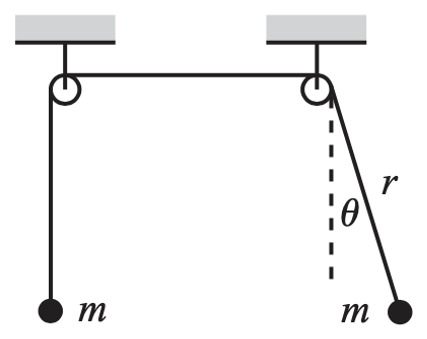
\includegraphics[width=0.4\textwidth]{Finala_P9.png}
    \label{P7}
\end{figure}

\subsection*{Answer}

\subsubsection*{(1) Kinetic Energy ($T$) [3 points]}
\begin{itemize}
    \item \textbf{Left Mass Kinematics:} \hfill \textbf{[1 point]} \\
    Identify that the left mass moves vertically with speed $\dot{r}$ (due to the string constraint).
    $$ T_{left} = \frac{1}{2}m\dot{r}^2 $$
    \item \textbf{Right Mass Kinematics:} \hfill \textbf{[2 points]} \\
    Identify the velocity squared of the right mass in polar coordinates ($v^2 = \dot{r}^2 + r^2\dot{\theta}^2$).
    $$ T_{right} = \frac{1}{2}m(\dot{r}^2 + r^2\dot{\theta}^2) $$
\end{itemize}

\subsubsection*{(2) Potential Energy ($V$) [3 points]}
\begin{itemize}
    \item \textbf{Right Mass Potential:} \hfill \textbf{[2 points]} \\
    Correctly expressing the gravitational potential of the swinging mass. Assuming the zero potential level is at the pulley:
    $$ V_{right} = -mgr \cos\theta $$
    \textit{Note: Sign errors deduct 1 point.}
    \item \textbf{Left Mass Potential:} \hfill \textbf{[1 point]} \\
    Correctly relating the height of the left mass to the coordinate $r$. Since the total string length is constant, if right length is $r$, left length is $L-r$.
    $$ V_{left} = -mg(L-r) \quad \text{or equivalent to} \quad V_{left} = +mgr $$
\end{itemize}

\subsubsection*{(3) The Lagrangian ($L$) [1 point]}
\begin{itemize}
    \item Constructing $L = T - V$ correctly using the terms derived above.
    $$ L = \frac{1}{2}m\dot{r}^2 + \frac{1}{2}m(\dot{r}^2 + r^2\dot{\theta}^2) - (mgr - mgr\cos\theta) $$
    Simplifying to:
    $$ L = m\dot{r}^2 + \frac{1}{2}mr^2\dot{\theta}^2 - mgr(1 - \cos\theta) $$
\end{itemize}

\subsubsection*{(4) Equations of Motion [5 points]}
Apply the Euler-Lagrange equation: $\frac{d}{dt}\left(\frac{\partial L}{\partial \dot{q}}\right) - \frac{\partial L}{\partial q} = 0$.

\begin{description}
    \item[A. Equation for $r$] \hfill \textbf{[3 points]}
    \begin{itemize}
        \item Derivatives:
        $$ \frac{\partial L}{\partial \dot{r}} = 2m\dot{r}, \quad \frac{d}{dt}\left(\frac{\partial L}{\partial \dot{r}}\right) = 2m\ddot{r} $$
        $$ \frac{\partial L}{\partial r} = mr\dot{\theta}^2 - mg + mg\cos\theta $$
        \item Final Equation:
        $$ 2m\ddot{r} - mr\dot{\theta}^2 + mg(1 - \cos\theta) = 0 $$
        Or simplified:
        $$ \boxed{2\ddot{r} = r\dot{\theta}^2 - g(1 - \cos\theta)} $$
    \end{itemize}

    \item[B. Equation for $\theta$] \hfill \textbf{[2 points]}
    \begin{itemize}
        \item Derivatives:
        $$ \frac{\partial L}{\partial \dot{\theta}} = mr^2\dot{\theta}, \quad \frac{d}{dt}\left(\frac{\partial L}{\partial \dot{\theta}}\right) = \frac{d}{dt}(mr^2\dot{\theta}) $$
        $$ \frac{\partial L}{\partial \theta} = -mgr\sin\theta $$
        \item Final Equation:
        $$ \frac{d}{dt}(mr^2\dot{\theta}) + mgr\sin\theta = 0 $$
        Or expanded/simplified:
        $$ \boxed{r\ddot{\theta} + 2\dot{r}\dot{\theta} + g\sin\theta = 0} $$
    \end{itemize}
\end{description}

\newpage

\section*{Problem 9 [$10$ points]}
Consider a particle of mass $m$ and electric charge $q$ moving in the presence of time-dependent electromagnetic fields. The particle's motion is described by the relativistic Lagrangian:
\[
L = -mc^2\sqrt{1 - \frac{v^2}{c^2}} + q\, \mathbf{v} \cdot \mathbf{A}(\mathbf{r}, t) - q\, V(\mathbf{r}, t),
\]
where $\mathbf{v} = \dv{\mathbf{r}}{t}$ is the particle's velocity; $V(\mathbf{r}, t)$ is the scalar potential; $\mathbf{A}(\mathbf{r}, t)$ is the vector potential; $c$ is the speed of light. Take the non-relativistic limit by expanding the Lagrangian to leading order in $v/c$ (i.e., assume $v \ll c$). From the resulting approximate Lagrangian, derive the Hamilton's equations of motion.
Hint: $\mathbf{E} = -\nabla V - \pdv{\mathbf{A}}{t}$ and $\mathbf{B} = \nabla \times \mathbf{A}$.

\subsection*{Answer}
\subsubsection*{(1) Non-Relativistic Approximation (3 points)}
\begin{itemize}
    \item Expand the relativistic term $\sqrt{1 - v^2/c^2}$ using the Taylor series $(1-x)^{1/2} \approx 1 - x/2$:
    \[
    -mc^2\sqrt{1 - \frac{v^2}{c^2}} \approx -mc^2\left(1 - \frac{v^2}{2c^2}\right) = -mc^2 + \frac{1}{2}mv^2
    \]
    \hfill \textbf{(1 point)}
    \item Write down the approximate non-relativistic Lagrangian. Note that the constant term $-mc^2$ can be dropped as it does not affect the equations of motion (though keeping it is also correct):
    \[
    L \approx \frac{1}{2}mv^2 + q\, \mathbf{v} \cdot \mathbf{A} - q\, V
    \]
    \hfill \textbf{(2 points)} \\
\end{itemize}

\subsubsection*{(2) Euler-Lagrange Derivatives (4 points)}
\begin{itemize}
    \item \textbf{Time Derivative Term:}
    Calculate the canonical momentum $\pdv{L}{\mathbf{v}}$ and its total time derivative.
    \[ \frac{\partial L}{\partial \mathbf{v}} = m\mathbf{v} + q\mathbf{A} \]
    Compute $\frac{d}{dt}(\frac{\partial L}{\partial \mathbf{v}})$, correctly applying the chain rule to $\mathbf{A}(\mathbf{r}, t)$:
    \[ \frac{d}{dt}(m\mathbf{v} + q\mathbf{A}) = m\dot{\mathbf{v}} + q\left( \frac{\partial \mathbf{A}}{\partial t} + (\mathbf{v} \cdot \nabla)\mathbf{A} \right) \]
    \hfill \textbf{(2 points)} \\

    \item \textbf{Spatial Derivative Term:}
    Calculate the gradient $\pdv{L}{\mathbf{r}}$. Use vector identity $\nabla(\mathbf{v} \cdot \mathbf{A}) = (\mathbf{v} \cdot \nabla)\mathbf{A} + \mathbf{v} \times (\nabla \times \mathbf{A})$ (treating $\mathbf{v}$ as constant independent of $\mathbf{r}$):
    \[ \frac{\partial L}{\partial \mathbf{r}} = q\nabla(\mathbf{v} \cdot \mathbf{A}) - q\nabla V = q\left[ (\mathbf{v} \cdot \nabla)\mathbf{A} + \mathbf{v} \times (\nabla \times \mathbf{A}) \right] - q\nabla V \]
    \hfill \textbf{(2 points)} \\
\end{itemize}

\subsubsection*{(3) Final Equation of Motion (3 points)}
\begin{itemize}
    \item \textbf{Assembly and Cancellation:}
    Equate the time derivative term to the spatial derivative term:
    \[ m\dot{\mathbf{v}} + q\frac{\partial \mathbf{A}}{\partial t} + q(\mathbf{v} \cdot \nabla)\mathbf{A} = q(\mathbf{v} \cdot \nabla)\mathbf{A} + q\mathbf{v} \times (\nabla \times \mathbf{A}) - q\nabla V \]
    Show that the term $q(\mathbf{v} \cdot \nabla)\mathbf{A}$ cancels out on both sides.
    \hfill \textbf{(1 point)}
    
    \item \textbf{Field Identification:}
    Rearrange the terms and substitute the definitions $\mathbf{B} = \nabla \times \mathbf{A}$ and $\mathbf{E} = -\nabla V - \pdv{\mathbf{A}}{t}$:
    \[ m\dot{\mathbf{v}} = q\left( -\nabla V - \frac{\partial \mathbf{A}}{\partial t} \right) + q\mathbf{v} \times (\nabla \times \mathbf{A}) \]
    \hfill \textbf{(1 point)}
    
    \item \textbf{Result:}
    Arrive at the Lorentz force law:
    \[ m\dot{\mathbf{v}} = q(\mathbf{E} + \mathbf{v} \times \mathbf{B}) \quad \text{or} \quad \mathbf{F} = q(\mathbf{E} + \mathbf{v} \times \mathbf{B}) \]
    \hfill \textbf{(1 point)}
\end{itemize}

\end{document}